\documentclass[11pt]{article}

% load some asm stuff -
\usepackage{amssymb}
\usepackage{amsmath}
\usepackage{amsthm}
%\usepackage{palatino,lettrine}
\usepackage{fancyhdr}
\usepackage{epsfig}
\usepackage[round,comma,sort]{natbib}
\usepackage{simplemargins}
\usepackage{setspace}
\usepackage{wrapfig}
\usepackage{hyperref}
%\usepackage{boiboites}
\usepackage[margin=0pt,font=small,labelfont=bf]{caption}

\bibliographystyle{plos2015}

% Set the size
%\textwidth = 6.75 in
%\textheight = 9.75 in
%\oddsidemargin = 0.0 in
%\evensidemargin = 0.0 in
%\topmargin = 0.01 in
%\headheight = 0.0 in
%\headsep = 0.25 in
%\parskip = 0.15in
\doublespace

\setallmargins{1in}

\newtheorem{example}{Example}[section]
\newtheorem{thm}{Theorem}[section]
\newtheorem{property}{Property}[section]

\theoremstyle{definition}
\newtheorem{defn}[thm]{Definition}

\makeatletter
\renewcommand\subsection{\@startsection
	{subsection}{2}{0mm}
	{-0.05in}
	{0.5\baselineskip}
	{\normalfont\normalsize\bfseries}}
\renewcommand\subsubsection{\@startsection
	{subsubsection}{2}{0mm}
	{-0.05in}
	{-0.5\baselineskip}
	{\normalfont\normalsize\itshape\bfseries}}
\renewcommand\paragraph{\@startsection
	{paragraph}{2}{0mm}
	{-0.05in}
	{-0.5\baselineskip}
	{\normalfont\normalsize\itshape}}
\makeatother
\linespread{1.2}

\fancypagestyle{proposal}{\fancyhf{}%
	\fancyhead[RO,LE]{\thepage}%
	\fancyhead[LO,RE]{CHEME 131 Module 1 Zero Coupon Treasury Securities}%
	\renewcommand\headrulewidth{1pt}}
\pagestyle{proposal}

\usepackage{mdframed}
\definecolor{lgray}{rgb}{0.92,0.92,0.92}
\definecolor{lsalmon}{rgb}{1.0,0.63,0.48}

% Single space'd bib -
\setlength\bibsep{0pt}

\renewcommand{\rmdefault}{phv}\renewcommand{\sfdefault}{phv}
%\newboxedtheorem[boxcolor=black, background=gray!5,titlebackground=orange!20,titleboxcolor = black]{color_box_example}{Example}{test}

% Change the number format in the ref list -
\renewcommand{\bibnumfmt}[1]{#1.}

% Change Figure to Fig.
\renewcommand{\figurename}{Fig.}

%Joycelyn Chan, Joshua Lequieu, Michael Paull, Chidanand Balaji, Ryan Tasseff
%Our derivation follows closely the earlier development of Fredrickson \citep{Fredrickson:1976fk}.

% Begin ...
\begin{document}

%\begin{titlepage}
{\par\centering\textbf{\Large CHEME 131 Module 1: Zero Coupon Treasury Securities}}
\vspace{0.2in}
{\par \centering \large{Jeffrey D. Varner$^{*}$}}
\vspace{0.1in}
{\par \centering \large{$^{*}$}R. F. Smith School of Chemical and Biomolecular Engineering}
{\par \centering \large{Cornell University, Ithaca NY 14853}}
% \vspace{0.1in}
% {\par \centering \small{Copyright \copyright\ Jeffrey Varner 2018. All Rights Reserved.}}\\

%\end{titlepage}
\date{}
\thispagestyle{empty}

\setcounter{page}{1}

% \begin{mdframed}[backgroundcolor=lgray]

% 	\subsection*{Background}
% 	We have discussed idealized reversible power generation and refrigeration cycles, and considered the impact of
% 	process irreversibility. In this lecture module, we will expand on the topic of irreversibility. In particular, we will develop expressions for
% 	the rate of \textit{lost work} caused by irreversibility in terms if the rate of entropy generation and process unit efficiencies.

% 	\vspace{0.1in}
% 	\subsection*{Student outcomes}
% 	At the end of this lecture module, students will be able to:
% 	\begin{itemize}
% 	  \item[O$_1$]{Describe the terms in the entropy balance for an open time dependent and steady-state system}
% 		\item[O$_2$]{Relate the rate of lost work $\dot{W}_{lost}$ to the rate of entropy generation $\dot{S}_{G}$ in a steady-state system.}
% 		\item[O$_3$]{Relate the efficiency of common equipment, e.g., pumps, compressors turbines etc to the rate of entropy generation $\dot{S}_{G}$ in a steady-state system.}
% 	\end{itemize}

% \end{mdframed}

% \clearpage

\section*{Introduction}
\href{https://www.investor.gov/introduction-investing/investing-basics/glossary/treasury-securities}{United States Marketable Treasury Securities}, 
are issued by the U.S. Department of the Treasury to fund its operations and meet financial obligations. 
These debt securities are structured loan agreements between a borrower, i.e., the U.S. government, and a lender (you) 
that allows the government to fund its operations and obligations (Fig. \ref{fig:govt-debt-schematic}).
The debt holder and the U.S. Treasury have a marketable repayment agreement, which can be held by the lender (you) until the completion of the contract or resold on a secondary market. Although there are various types of U.S. government debt securities, they all share a few common characteristics. 
First, U.S. Treasury debt securities have a predetermined term length; thus, the contract duration between the borrower and lender is fixed.
Second, U.S. Treasury debt securities have a par value, representing the instrument's face value, a price (which may differ from the par value), and an interest rate paid to the lender. Next, some U.S. Treasury debt securities have interest payments commonly called coupons. These payments give the lender fixed cashflows on a predetermined schedule throughout the debt instrument's term. Finally, income from interest on U.S. Treasury debt securities is free of state and local income taxes but subject to federal income taxes.
You can purchase U.S. Treasury debt directly from the \href{https://www.treasurydirect.gov/indiv/products/prod_tbonds_glance.htm}{United States Treasury via TreasuryDirect} 
or through a bank or broker to lend money to the U.S. government.

\begin{figure}[h]
    \centering
    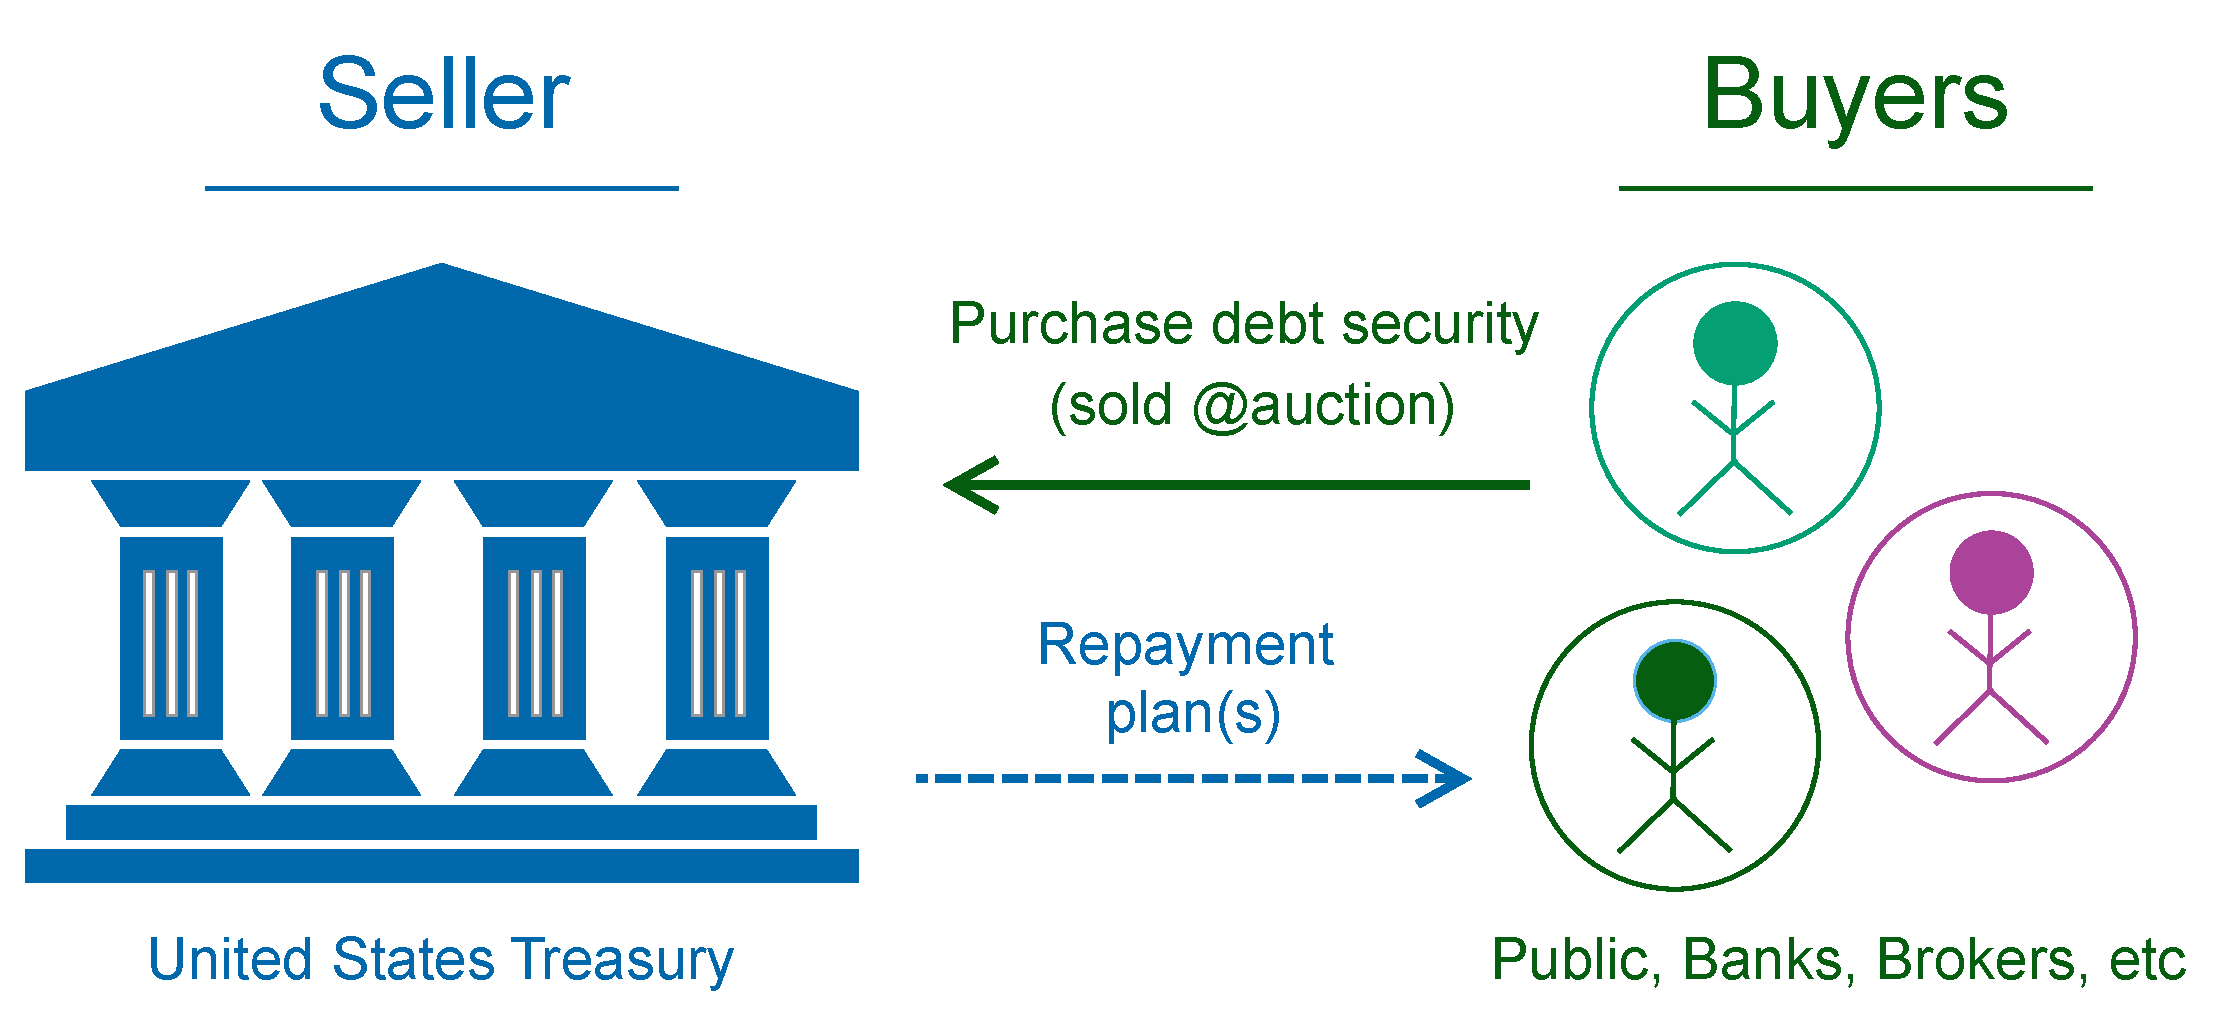
\includegraphics[width=0.85\textwidth]{./figs/Fig-Govt-Debt-Schematic.pdf}
    \caption{Schematic of U.S. Government Debt Securities. }\label{fig:govt-debt-schematic}
\end{figure}


\section*{Treasury Bills, Notes and Bonds}\label{sec:treasury-bills}
\href{https://treasurydirect.gov/marketable-securities/treasury-bills/}{United States Treasury Bills}, or T-bills are Treasury debt instruments with short-term maturity periods T = 4, 8, 13, 26, and 52 weeks and zero coupon payments
Thus, Treasury bills (T-bills) are short-term debt securities issued by the U.S. Treasury. \href{https://treasurydirect.gov/marketable-securities/treasury-notes/}{United States Treasury Notes or T-notes}, 
are debt instruments that provide a stable interest payment every six months until maturity, called a coupon payment.
These notes are offered in terms of T = 2, 3, 5, 7, and 10 years and can be bought for more or less than their face (par) value. 
Upon maturity, the lender receives the entire par value. 
\begin{figure}[h]
    \centering
    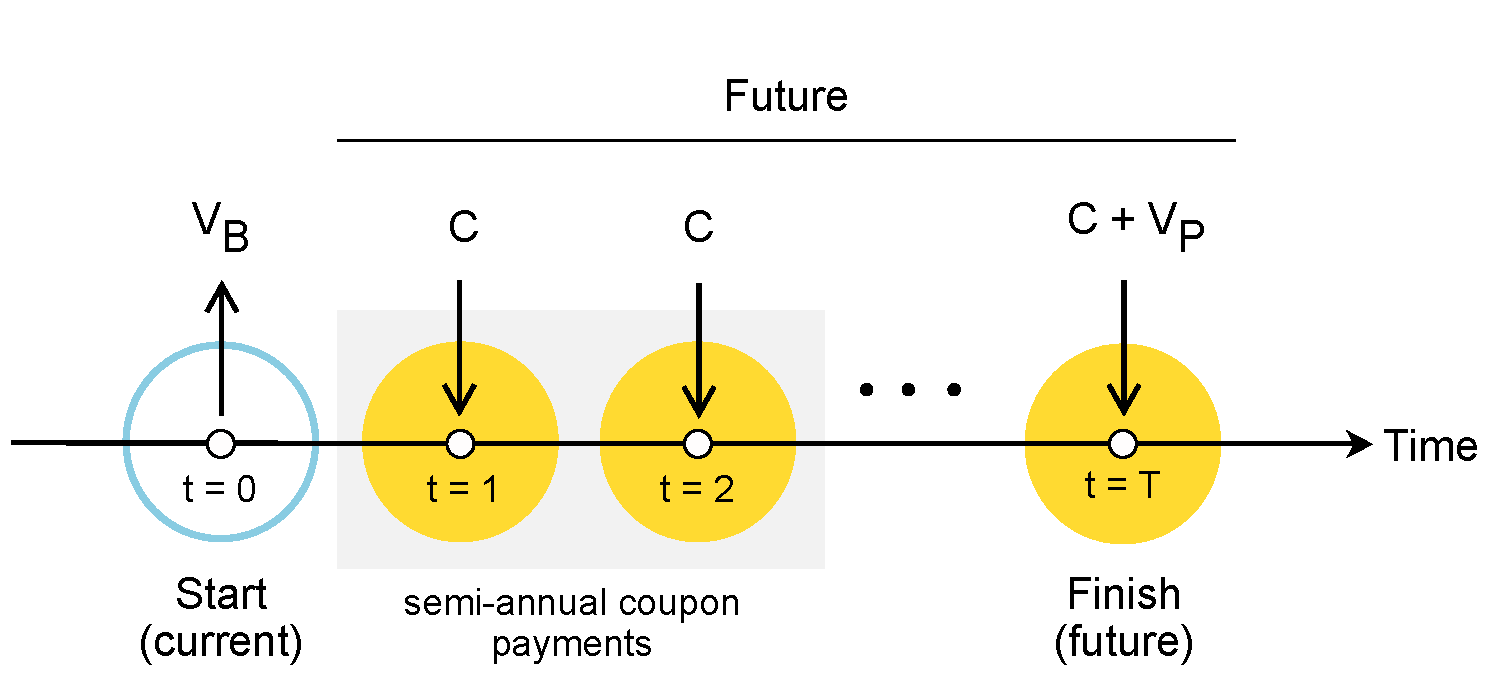
\includegraphics[width=0.75\textwidth]{./figs/Fig-Bond-Asset-Timeline-Schematic.pdf}
    \caption{Asbtract asset schematic of coupon-bearing Treasury note (bond). The lender (you) gives the United States Treasury 
    the price $V_{B}$ of the note (bond) at auction. In return, the Treasury pays semi-annual coupon paymemts to holder (you) 
    over the life of the note (bond). At maturity, the lender (you) receives the final coupon payment
    and the par value of the note (bond). Schematic written from the note (bond) holders perspective.}\label{fig:govt-note-bound-schematic}
\end{figure}
\href{https://treasurydirect.gov/marketable-securities/treasury-bonds/}{Treasury notes and bonds} are coupon debt instruments, which means that the lender receives periodic interest payments based on a coupon rate during the lifespan of the security. 
The coupon rate is fixed at the time of issuance and is calculated as a percentage of the par value. 
At maturity, the lender receives the par value of the bond (or note) and a final coupon payment.

\section*{Pricing Zero-Coupon Treasury Securities}\label{sec:zero-coupon-treasury-securities}
The price of a zero-coupon Treasury bill $V_{B}$ with an effective interest rate of $\bar{r}$ and a maturity of \texttt{T}-years at auction 
is the discounted face (par) value $V_{P}$ such that the net present value (NPV) of the bill is zero:
\begin{equation}    
\text{NPV}(T,r) = -V_{B} + \mathcal{D}_{T,0}^{-1}(\bar{r})\cdot{V_{P}} = 0
\end{equation}
or equivalently:
\begin{equation}
    V_{B} = \mathcal{D}_{T,0}^{-1}(\bar{r})\cdot{V_{P}}
\end{equation}
The quantity \texttt{T} denotes the duration of the bill (in years), 
$\bar{r}$ is the effective annualized interest rate,  and $\mathcal{D}_{T,0}^{-1}(\bar{r})$ is the inverse multistep discount factor
for period $0\rightarrow{T}$. 
The discount factor $\mathcal{D}_{T,0}^{-1}(\bar{r})$ can be either computed on a discrete or continuous basis. 
In the case of treasury securities, the discount factor is computed on a discrete basis, assuming $m$ compounding periods per year.

\subsection*{Multiperiod Discrete Discount Factor}
Fill me in.



\end{document}
